%\documentclass[11pt,a4paper,titlepage,twoside]{article}
\documentclass[12pt,a4paper,twoside]{article}
\usepackage{mystyle}
%\usepackage{gplot}
%\usepackage{foto_v001}
%\usepackage{mechanik_v001}

%\author{Felix Binder}
\title{Kernphysik}
\date{}

\newcommand{\Kern}[3]{$^{#1}_{\phantom{1}#2}\text{#3}$}
\begin{document}
\maketitle

\section*{Einführung}
Die Kernphysik gehört zu den neueren Entwicklungen der Physik und beschäftigt sich, wie der Name schon sagt, mit den Kernen der Atome.
Jedes Atom besitzt einen elektrisch positiven Kern um den elektrisch negativ geladene Elektronen kreisen. Ein neutrales Atom besitzt gleich
viele positive Ladungen im Kern wie negative Ladungen in seiner Hülle.
Die Elektronen, besonders die in der äusseren Hülle bestimmen die chemischen Eigenschaften des Atoms.

Der Kern besteht aus \emph{Nukleonen}, so nennt man die Teilchen, die den Kern bilden. 
Es sind elektrisch positiv geladenen \emph{Protonen} und elektrisch neutrale \emph{Neutronen}.
Die Anzahl $Z$ der Protonen bestimmt die Art des Atoms, ein Atom mit acht Protonen ist zum Beispiel immer ein Sauerstoffatom.
Gleichnamige Ladungen stossen sich ab, deshalb braucht der Atomkern Neutronen, um die abstossende Wirkung der Protonen zu kompensieren.
Ohne diese wäre der Kern nicht stabil.
Die Anzahl der Neutronen in einem Kern wird mit $N$ angegeben.
Die Summe von Ordungszahl $Z$ und Neutronenzahl $N$ nennt man Massenzahl $A$.
Kern mit gleicher Ordungszahl und unterschiedlicher Massenzahl nennt man \emph{Isotope}.

In leichten Kernen sind etwa gleich viele Protonen wie Neutronen. 
Schwere Kerne hingegen haben mehr Neutronen als Protonen.

\begin{aufgabe}
	Ordnen Sie die folgenden Entdeckungen in die Zeitleiste ein.
Das Element mit Ordungszahl $Z=110$ wurde erzeugt,
Entdeckung der erste Kernspaltung durch Otto Hahn,
Entdeckung des Radiums durch Marie Curie,
Entdeckung des Atomkerns durch Ernest Rutherford,
Das Neutrino wird durch Wolfgang Pauli theoretisch vorausgesagt,
Entdeckung des Neutrons,
Entdeckung der Radioaktivität,
Experimentelle Bestätigung des Antiprotons,
Experimentelle Bestätigung des Neutrino,
Spezielle Relativitätstheorie durch Albert Einstein ($E=m\cdot c^2$),
Experimentelle Bestätigung des Higgs-Teilchens.
Quarks werden entdeckt,
\end{aufgabe}

\begin{aufgabe}
	Um den Atomkern zu beschreiben, wird häufig ein Tröpfchenmodel benutzt. Dabei nimmt man an, dass sich der Atomkern wie ein Wassertropfen verhält.
	\begin{enumerate} [a)]
		\item Zeichnen Sie drei unterschiedlich geformte Wassertropfen.
		\item Welche Tropfenform hat die niedrigste Energie?
	\end{enumerate}
\end{aufgabe}

\newpage

\newcommand{\LS}[2]{
\pgfmathsetmacro{\Datum}{0.1*(#1-1814)};
%\draw (\Datum,-0.1) -- (\Datum,0.1) node [rotate=90, left] {#2};
\draw (\Datum,-0.1) -- (\Datum,0.1) node [left] {#2};
}

\newcommand{\RS}[2]{
\pgfmathsetmacro{\Datum}{0.1*(#1-1814)};
%\draw (\Datum,0.1) -- (\Datum,-0.1) node [rotate=90, right] {#2};
%\path (\Datum,0.1) -- (\Datum,-0.1) node [right] {\phantom{#2}};
\draw (\Datum,0.1) -- (\Datum,-0.1) node [right] {#2};
}

\begin{tikzpicture}[rotate=90]
	
%Zeitleiste
\draw [->] (0,0)--(21,0);
\LS{1876}{Erstes Telefon}
\LS{1847}{Erste schweizer Eisenbahnstrecke}
\LS{1886}{Erstes Auto}
\LS{1896}{Erstes Röntgenbild}
\LS{1973}{Magnetresonanztomographie}
\LS{1945}{Zündung der ersten Atombombe}
\LS{1956}{Test einer Wasserstoffbombe}
\LS{1992}{Erstes modernes Mobilfunktelefon}
\LS{1969}{Die ersten Menschen auf dem Mond}
\LS{2007}{Erstes IPhone}
\LS{1826}{Erstes Foto der Welt}

%\RS{1895}{Entdeckung der Röntgenstrahlen}
\RS{1896}{Entdeckung der Radioaktivität}
\RS{1898}{Entdeckung des Radiums durch Marie Curie}
\RS{1905}{Spezielle Relativitätstheorie durch Albert Einstein ($E=m\cdot c^2$)}
\RS{1909}{Entdeckung des Atomkerns durch Ernest Rutherford}
\RS{1930}{Das Neutrino wird durch Wolfgang Pauli theoretisch vorausgesagt}
\RS{1932}{Entdeckung des Neutrons}
\RS{1938}{Entdeckung der erste Kernspaltung durch Otto Hahn}
\RS{1955}{Experimentelle Bestätigung des Antiprotons}
\RS{1956}{Experimentelle Bestätigung des Neutrino}
\RS{1968}{Quarks werden entdeckt}
\RS{1994}{Das Element mit Ordungszahl $Z=110$ wurde erzeugt}
\RS{2013}{Experimentelle Bestätigung des Higgs-Teilchens}
\end{tikzpicture}


\newpage

\section*{Bindungsenergie}

Auszug aus dem Wikipediaartikel: Bindungsenergie zu finden unter \\
http://de.wikipedia.org/wiki/Bindungsenergie (11.01.14)

Bindungsenergie muss aufgebracht werden, um ein gebundenes System aus zwei oder mehr Bestandteilen 
(beispielsweise einen Himmelskörper, ein Molekül, ein Atom, einen Atomkern), die durch Anziehungskräfte 
zusammengehalten werden, in seine Bestandteile zu zerlegen. Eine ebenso große Energie wird freigesetzt, 
wenn sich das gebundene System aus den Einzelteilen bildet. Manchmal wird unter Bindungsenergie nicht diese 
Energiemenge selbst, sondern die Änderung des Energieinhalts des Systems verstanden, wenn seine Teile sich 
miteinander verbinden; dann hat sie den gleichen Betrag, ist aber negativ. So ist z. B.\ die in der Chemie 
gebräuchliche Reaktionsenthalpie $\Delta H$ negativ, wenn bei der Reaktion Energie frei wird.

Die Bezeichnung Bindungsenergie ist ein gängiger Fachausdruck, aber sprachlich etwas unglücklich gewählt. 
Sie führt -- besonders mit einem nachfolgenden Genitiv, wie z. B. Bindungsenergie ``des Uran-Atomkerns'' oder ``des ATP-Moleküls'' -- 
leicht zu dem Missverständnis, es handele sich um einen Energiebetrag, der in dem gebundenen System vorhanden 
ist und aus ihm freigesetzt werden kann. Richtig ist, wie oben gesagt, das Gegenteil: 
die Bindungsenergie ist bereits bei der Bildung des gebundenen Systems freigesetzt und abgegeben worden, ist also nun nicht mehr verfügbar.

\subsection*{Veranschaulichung}

Wenn beispielsweise der Abstand zweier Dauermagnete hinreichend gering ist, ziehen sie einander an und bewegen sich aufeinander zu. 
Augenblicke vor dem Zusammenstoß besitzen beide Magnete ihre höchste kinetische Energie, welche dann in Schallenergie und Wärme umgewandelt wird. 
Um die Magnete wieder voneinander zu trennen muss die Bindungsenergie aufgebracht werden, sie stimmt vom Betrag her mit der freigesetzten 
Gesamtenergie überein. Möchte man also die Magnete voneinander trennen, muss die Bindungsenergie in das System eingebracht werden. 
Wird dies nicht getan, so bleiben die Magnete vereint.

\subsection*{Kernphysik}

In der Kernphysik ist die Bindungsenergie die Energiemenge, die aufgewandt werden muss, um den Atomkern in seine Nukleonen zu zerlegen. Umgekehrt wird eine ebenso große Energie frei, wenn sich Nukleonen in einem Kern vereinigen.

Die Bindung kommt durch die anziehende Kraft der starken Wechselwirkung zwischen den Nukleonen zustande. Sie wird durch die gegenseitige Coulomb-Abstoßung der elektrisch positiv geladenen Protonen im Kern geschwächt. Die maximale Bindungsenergie pro Nukleon wird bei Nickel-62 erreicht. Leichtere Kerne haben relativ mehr Nukleonen an der Oberfläche, wo sie schwächer gebunden sind. Bei schwereren Kernen nimmt die Bindungsenergie je Nukleon dann wieder ab, denn je mehr Protonen vorhanden sind, desto stärker wächst die abstoßende Coulombkraft zwischen ihnen an. Daher kann im Gebiet der leichten Kerne durch Kernverschmelzung (Kernfusion), im Gebiet der schweren Kerne durch Kernspaltung Energie gewonnen werden. Die Bindungsenergie von Atomkernen kann im Rahmen des Tröpfchenmodells mit der Bethe-Weizsäcker-Formel abgeschätzt werden. Die Zacken in der Grafik hängen mit den Magischen Zahlen zusammen.

Die Bindung ist wegen der Äquivalenz von Masse und Energie mit einem Massendefekt verbunden: Der gebundene Kern hat zwischen \SI{0,1}{\percent} (Deuteron)
und \SI{0,9}{\percent} (Ni-62) weniger Masse als alle seine Nukleonen zusammengenommen. Aus einer genauen Bestimmung der Masse $M$ eines Atoms 
lässt sich daher die Bindungsenergie $E_{\text{B}}$ des Kerns ableiten:

\begin{eqnarray*}
    E_{\text{B}}(Z,A) = \left(Z \cdot m_{\text{p}} + Z \cdot m_{\text{e}} + (A - Z) \cdot m_{\text{n}} - m(A,Z)\right) \cdot c^2
\end{eqnarray*}

Dabei ist\\
	$m(A,Z)$ die Masse des Atoms,\\
	$A$ seine Massenzahl,\\
	$Z$ seine Ordnungszahl,\\
	$m_{\text{p}}$ die Masse eines freien Protons,\\
	$m_{\text{n}}$ die Masse eines freien Neutrons,\\
	$c$ die Lichtgeschwindigkeit.

Die Bindungsenergie kurzlebiger Kerne lässt sich beispielsweise durch Messung der Energien ihrer Zerfallsprodukte bestimmen.

\begin{center}
	\includegraphics[width=0.90\textwidth]{./Binding_energy_curve_-_common_isotopes_DE.pdf}
\end{center}


\newpage

\begin{aufgabe}
	Lesen Sie den Artikel zur Bindungsenergie aus der Wikipedia und beantworten Sie folgende Fragen:
	\begin{enumerate} [a)]
		\item Beschreiben Sie in zwei Sätzen was die Bindungsenergie ist.
		\item Welche Wechselwirkung hält die Atomkerne zusammen?
		\item Wie erklärt der Artikel die relativ schwache Bindung der leichten Kerne?
		\item Welcher Kern hat die höchste Bindungsenergie pro Nukleon im Atomkern? Wie hoch ist diese Energie in Joule?
		\item Warum kann man die Bindungsenergie kurzlebiger Kerne aus deren Zerfallsprodukten bestimmen?
		\item Wo in der Grafik stehen die Kerne, die sich fusionieren lassen? Wo die, die bei der Spaltung Energie freigeben? Können Sie das erklären?
	\end{enumerate}
\end{aufgabe}

\begin{aufgabe}
 In der Grafik ist $^3_2\text{He}$ und $^3_1\text{H}$ aufgeführt. Welches der beiden sollte stabiler sein? Stimmt das?
\end{aufgabe}

\begin{aufgabe}
	Berechnen Sie mit Hilfe der Grafik die Bindungsenergie des \Kern{16}{8}{O} Kerns.
\end{aufgabe}


\begin{aufgabe}
	Nehmen Sie an ein Kern der Massenzahl $A=240$ wird in zwei Kerne der mit der Massenzahl $A=120$ gespalten. Bestimmen Sie aus der Grafik die dabei
	freiwerdende Energie.
\end{aufgabe}

\begin{aufgabe}
	In der Sonne werden Wasserstoffkerne zu Heliumkernen fusioniert.
	Wie viel Energie wird dabei frei. Benutzen Sie die Grafik zum Lösen der Aufgabe.
\end{aufgabe}

\newpage

\section*{Radioaktivität}

Die Aufgaben auf dieser Seite sind als Ergänzung des Kapitels 2: Radioaktivität, des Leitprogramms ``Radioaktivität'' der ETH Zürich zu verstehen.
Das vollständige Leitprogramm können Sie unter http://www.educ.ethz.ch/unt/um/phy/mp/radioakt/index finden.

\begin{aufgabe}
	C-11 ist ein $\beta^{+}$-Strahler. In welches Element wandelt sich das Kohlenstoff durch den Zerfall?
\end{aufgabe}

\begin{aufgabe}
	Das Bild zeigt einen Ausschnitt aus einer Nuklidkarte. 
	Zeigen Sie durch Pfeile, wohin das Mutternuklid durch $\alpha$-, $\beta^{-}$- und $\beta^{+}$-Zerfall zerfällt?

	\begin{center}
		
	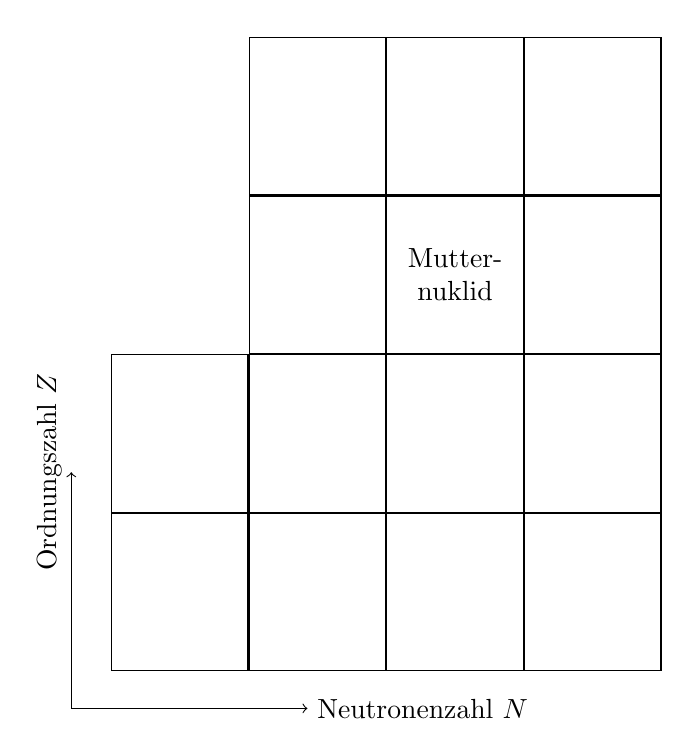
\begin{tikzpicture}
\matrix (N)[every node/.style={draw, text width=1.5cm, align=flush center, minimum height=2cm}]
{
& \node (){}; & \node {}; & \node {}; \\
& \node (){}; & \node {Mutter-nuklid}; & \node {}; \\
\node {}; &\node (){}; & \node {}; & \node {}; \\
\node (UL) []{}; &\node (){}; & \node {}; & \node {}; \\};
\draw [->](-4,-4.5) --++(0:3cm) node [right] {Neutronenzahl $N$};
\draw [->](-4,-4.5) --++(90:3cm) node [rotate=90, above] {Ordnungszahl $Z$};
	\end{tikzpicture}
	\end{center}

\end{aufgabe}

\begin{aufgabe}
	Die Isotope, die in der Isotopenkarte links von den stabilen Isotope stehen, sind oft $\beta^{+}$-Strahler.
	Die Isotope rechts der stabilen Isotope sind oft $\beta^{-}$-Strahler. Wie können Sie sich das erklären?
\end{aufgabe}

\begin{aufgabe}
	Beim Zerfall eines Radium-222 Kerns in einen Radon-118 Kern wird ein Heliumkern frei ($\alpha$-Strahler).
	Welche Geschwindigkeit hat der Heliumkern? \\
	Tipp: Es gilt Energieerhaltung.\\
	\Kern{222}{88}{Ra}: \SI{222.0153618}{u}\\
	\Kern{218}{86}{Rn}: \SI{218.0055863}{u}\\
	$^4_2\text{He}$: \SI{4.0026032}{u}
\end{aufgabe}


\end{document}
